\documentclass[12pt, a4paper, openany]{book}
\usepackage{fstyle}

\graphicspath{ {./img/} }

\begin{document}
\title{Esami di Analisi Matematica}
\author{Fabio Ferrario}
\date{2022}
\maketitle
\tableofcontents

\chapter{Introduzione}
\section{Gli esami}
La professoressa Pini ha fornito, tramite E-Learning alcune prove d'esame degli anni precedenti:
\paragraph*{}
\begin{tabular}{ |c|c|c|c| }
	\hline
	Esame         & Crocette   & Domande Aperte & Note                       \\
	\hline
	Febbraio 2019 &            &                &                            \\
	Giugno 2019   & \checkmark &                &                            \\
	Luglio 2019   &            &                &                            \\
	Gennaio 2020  &            &                &                            \\
	Febbraio 2020 & \checkmark &                &                            \\
	Giugno 2020   & \checkmark &                & 1 parziale e 2 non risolte \\
	Luglio 2020   &            &                &                            \\
	Gennaio 2021  &            &                &                            \\
	Febbraio 2021 &            &                &                            \\
	Giugno 2021   & \checkmark &                &                            \\
	Luglio  2021  &            &                &                            \\
	Gennaio 2022  &            &                &                            \\
	Febbraio 2022 &            &                &                            \\
	\hline
\end{tabular}

\chapter{Compitini}
\section{Compitino 2019}
\subsection{Domande Chiuse}

\domanda{1a}{La serie $\serie{1}{+\infty} \frac{ln^4n}{n^{\alpha - 2} + 2n}$ è}
\risposta{Convergente sse $\alpha > 3$}
\spiegazione{
	$\frac{ln^4n}{n^{\alpha - 2} + 2n} = \frac{1}{ln^{-4}n\cdot n^{\alpha-2}+2n} $,  se $\alpha >3$ l'esponente di $n$ è $>1$ rendendo la serie convergente
}

\domanda{1b}{La serie $\serie{1}{+\infty} \frac{ln^3}{n^{\alpha - 1} + 3n}$ è}
\risposta{Convergente sse $\alpha > 2$}
\spiegazione{La serie diventa divergente se $\alpha = 2 \lor \alpha \leq 2$}

\domanda{2a}{La somma della serie $\serie{0}{+\infty} 3\cdot (-\frac{1}{2})^{n+1}$ è uguale a}
\risposta{$-1$}
\spiegazione{
	Una serie di tipo $\sum q^n$ con $q^n < 1$ è una serie geometrica, risolvibile quindi come $\frac{1}{1-q}$
}
\domanda{2b}{La somma della serie $\serie{0}{+\infty} 3\cdot (-\frac{1}{2})^{n+2}$ è uguale a}
\risposta{$\frac{1}{2}$}

\domanda{3a}{Il $\limite{n}{+\infty} \frac{3n^2-n+n ln n +(-1)^n}{2n+4n ln n - n^ - \frac 2/n^2}$ vale}
\risposta{3}


\chapter{Esami}
\section{Febbraio 2021}

\domanda{1}{Sia $a_n = \frac{n \ln (1- \frac{2}{n^3})}{n \sqrt[3]{n} - n^3}$. Allore, per $n \to +\infty$,
}
\risposta{$a_n \sim \frac{2}{n^5}$}
\spiegazione{
	$$
		a_n = \frac{n \ln(1-\frac{2}{n^3})}{n \sqrt[3]{n}-n^3} \rightarrow \frac{\frac{2}{n^2}}{n^3} \rightarrow \frac{2}{n^2} \cdot \frac{1}{n^3} = \frac{2}{n^5}
	$$
	Bisogna trovare una successione asintoticamente equivalente sia per il numeratore, che per il denominatore.
}
\domanda{2}{Sia $f:\R \to \R$ con $f'(0)=0,f''(x)=ln(e+x)$.Allora $f$ ha in $x=0$}
\risposta{Un punto di minimo Relativo}
\irrisolta

\domanda{3}{Sia $f:\R \to \R$ una funzione continua e dispari. Allora, $\int_{-3}{4} f(x) dx$ è uguale a}
\risposta{$\int_{3}^{4} f(x) dx$}
\spiegazione{Una funzione dispari è una funzione che ha il grafico simmetrico rispetto all'origine, quindi ha $f(-a) = -f(a)$.
	L'integrale è l'area sottesa della funzione \emph{con il segno}, quindi in una $f(x)$ dispari $\int_{-a}^{a} f(x) dx = 0$ (Spiegazione negli appunti).
	Di conseguenza è intuibile che in questa funzione l'integrale da -3 a 3 si annulla, e rimane solo l'area da 3 a 4.}


\domanda{4}{La derivata della funzione $f(x) = \sqrt[3]{\frac{x^3}{2} +1}$ è}
\risposta{$\frac{x^2}{2\sqrt[3]{(\frac{x^3}{2}+1)^2}}$}
\spiegazione{
	La derivata di una funzione composta è: $f(g(x))' = f'(g(x))\cdot g'(x)$.
	Per quanto riguarda la radice, è meglio farla a mano trasformandola ($\sqrt[\alpha]{x^\beta} = x^\frac{\beta}{\alpha}$).
	Il resto sono calcoli Algebrici
}

\domanda{5}{la serie $\serie{1}{+\infty} \frac{1}{n^{(\alpha+1)/2}\ln^2n}$ }
\risposta{Converge sse $\alpha \geq 1$}
\spiegazione{Siccome $n^{...}$ si moltiplica al logaritmo, se fosse infinitesimo annullerebbe il denominatore rendendo la serie divergente a infinito.
	Quindi, l'esponente di alpha deve essere positivo, di conseguenza $\alpha \geq 1$}


\domanda{6}{La funzione $f(x) = \begin{cases}a \sin x - b^2  & -2 \leq x \leq 0 \\ 1-e^x &0<x\leq 3\end{cases}$ è derivabile in $x=0$ se e solo se:}
\risposta{$a=-1,b=0$}
\spiegazione{
	Una funzione è derivabile in un punto se è continua e se i limiti destro e sinistro della derivata in quel punto coincidono.
	\\Verificando la continuità, è banale che $b^2=0 \to b=0$.
	\\Verficiando i limiti della derivata invece:
	$ f(x) = a sinx \implies f'(x) = a cos(x)$, $\limite{x}{o^-} a cos(x) = a$.
	\\ $f(x) = 1 -e^x \implies f'(x) = -e^x$, $\limite{x}{o^+} -e^x = -1$.
	\\Di conseguenza, $a = -1$ per la derivabilità.
}


\domanda{7}{Quali tra questi insiemi è un intervallo?}
\risposta{$\{x \in \R: 2|x| \geq x^2\}$}
\spiegazione{}

\domanda{8}{Date le funzioni $f(x) = \ln(x), g(x)= x^3, h(x) = 2-x$, la funzione composta $(h \circ g \circ f)(x)$ è:}
\risposta{$2-\ln(x)$}
\spiegazione{$(h \circ g \circ f)(x) = h(g(f(x)))$}


\section{Giugno 2019}

\domanda{1}{La serie $\serie{1}{+\infty}(-1)^n sin(\frac{3}{n^2})$}
\risposta{Converge assolutamente}
\spiegazione{
	Siccome abbiamo sia $(-1)^n$, che una successione $\sin(a_n)$, sappiamo che questa serie è a \emph{segno variabile}.
	\\Usiamo quindi il criterio dell'assoluta convergenza.
	$$
		|\serie{1}{+\infty}(-1)^n sin(\frac{3}{n^2})| = |sin(\frac{3}{n^2})| \sim \frac{3}{n^2}
	$$
	la corrispondenza asintotica vale perchè l'argomento del seno è infinitesimale.
	La successione risultante è una serie armonica di grado $> 1$, quindi converge.
}
\domanda{2}{La Successione $a_n = \frac{\ln(2+n^3)-5\sqrt[]{n^2-n}+2^{-n^4+5n}}{5n+3\ln n - n \ln n}}$ per $n \to +\infty$ ha limite:
\risposta{$\limite{n}{+\infty} = 0$}
\spiegazione{
	Si trova una successione asintoticamente equivalente sia per numeratore, che per denominatore.
	$$ a_n \sim \frac{2^{-n^4}}{5n}$$
	Si noti che nel numeratore, $2^{-n^4 +5n}$ il $+5n$ è "sovrastato" da $-n^4$, quindi è ignorabile.
	\\Siccome al numeratore abbiamo un valore infinitesimo,($ = (\frac{1}{2})^{n^4}$), la successione tende a $0$
}

\domanda{3}{La funzione $f(x) = \frac{2x^3+4x}{2-x^2} + e^{-\frac{1}{x}}$, per $x\to +\infty$, ha asintoto obliquo di equazione:}
\risposta{$$y=-2x+1$$}
\spiegazione{
	Per trovare un asintoto obliquo bisogna trovare $m$ e $q$ che compongono la retta $y=mx +q$:
	\\$
	m=\limite{x}{+\infty}\frac{f(x)}{x}
	= \frac{\frac{2x^3+4x}{2-x^2} + e^{-\frac{1}{x}}}{x}
	= (\frac{2x^3+4x}{2-x^2} + e^{-\frac{1}{x}})\cdot \frac{1}{x}
	= \frac{2x^3+4x}{2x-x^3} + \frac{e^{-\frac{1}{x}}}{x}
	= \frac{\cancel{x}(2x^2+4)}{\cancel{x}(2-x^2)} + \frac{e^{-\frac{1}{x}}}{x}
	\sim \frac{2\cancel{x^2}}{-\cancel{x^2}} + \frac{e^{-\frac{1}{x}}}{x}
	= -2 + \frac{e^{-\frac{1}{x}}}{x}
	$. Siccome $\frac{e^{-\frac{1}{x}}}{x}$ tende a $0$, allora $m$ equivale a $-2$
		\\Adesso dobbiamo trovare $q$
		\\$
		q = \limite{x}{+\infty} [f(x) -mx]
		= \frac{2x^3+4x}{2-x^2} + e^{-\frac{1}{x}} +2x
		\sim \frac{2\cancel{x^3}}{-\cancel{x^2}} + e^{-\frac{1}{x}} +2x
		=\cancel{-2x} + e^{-\frac{1}{x}} \cancel{+2x} = e^{-\frac{1}{x}} = 1
	$
	\\Quindi, l'asintoto obliquo esiste e ha equazione $y=-2x+1$
}

\domanda{4}{Sia $f(x) = \sqrt{x^2 +2x +3}$. allora $f'(1)$ vale:}
\risposta{$\frac{2}{\sqrt{6}}$}
\spiegazione{
	Basti ricordarsi che:
	\\La derivata di una radice è: \derivata{\sqrt[\alpha]{x}}{\frac{1}{\alpha \sqrt[\alpha]{x}}}
	\\Questa funzione è una funzione composta ($f(x) = \sqrt{g(x)}$), quindi bisogna derivarla come tale: $f(g(x)) = f'(g(x)) \cdot g'(x)$.
	\\Una volta calcolata la derivata e semplificata fino a un punto "comodo", basta sostituire $x$ con 1.
}

\domanda{5}{L'insieme delle soluzioni della disequazione $e^x \sqrt[3]{x-1} \geq 1$ è del tipo}
\risposta{$(\alpha, +\infty)$ con $\alpha>1$}
\spiegazione{
	Ci si chiede l'intervallo dei valori di $x$ per cui la disequazione è sostanzialmente "corretta", quindi quando il termine sinistro è maggiore di 1.
	\\Se si prova un po per esclusione, si vede che per $x=0$ è "falsa" e rimane così anche per valori minori di 0.
	\\$x=1$ ci da 0, quindi deve essere per forza un valore maggiore di 1
}

\domanda{6}{la funzione $f(x) = \ln(x^2+2x+3)$ è monotona crescente se e solo se}
\risposta{$x\in (-1,+\infty)$}
\spiegazione{
	Per trovare se una funzione è \emph{monotona crescente} bisogna porre la derivata della funzione $\geq 0$.
	Il risultato è $x\geq -1$, che equivale a $x\in (-1,+\infty)$.
}
\domanda{7}{L'estremo inferiore della successione $\{a_n\}_{n\geq0}$, dove $a_n = 3^{n+(-1)^nn}$ è:}
\risposta{
	1
}
\spiegazione{
	Per vedere l'estremo inferiore di una successione bisognerebbe provare qualche valore di $n$ a partire dal più piccolo (in questo caso 0).
	Se il termine è infinitesimale, l'estremo inferiore si trova con il limite, altrimenti vedi il valore minore che trovi.
}
\domanda{8}{$\int_{\pi/2}^{\pi} x \sin x dx$ vale:}
\risposta{
	$\pi -1$
}
\spiegazione{
	Integro per parti, quindi abbiamo:
	\\$f(x) = x$ e quindi $f'(x) = 1$
		\\$g'(x)= \sin(x)$ e quindi $g(x) = -\cos(x)$
	\\Risolvo con la formula dell'\emph{integrazione per parti}:
	$$x (-\cos(x)) - \int 1(-\cos(x)) = -x\cos(x)+\sin(x) = \sin(x)-x\cos(x)$$
	Risolvo l'integrale per gli estremi dati:
	$F(\pi) = \pi$, $F(\pi/2)=1$.
	Quindi l'integrale dato vale $\pi -1$
}

\subsection{Domande Aperte}
\domandaaperta{1i}{Data la serie $\serie{1}{+\infty} (\frac{x^2+6}{5x})^n$, Si determino i valori di $x\in\R \backslash \{0\}$ per cui converge, e se ne calcoli la somma.}

\rispostaaperta{
	La serie è di tipo gemoetrico con ragione $q=\frac{x^2+6}{5x}$, e per convergere deve essere $|q|<1$.
	$$|\frac{x^2+6}{5x}| < 1 = \frac{x^2+6}{|5x|}<1$$
	Risolviamo quindi per $x<0$ e per $x>0$.
	\begin{equation*}
		\begin{cases}
			x>0 \\
			\frac{x^2+6}{5x} < 1 = \frac{x^2+6}{5x} -1 < 0 =\frac{x^2+6-5x}{5x} < 0
		\end{cases}
	\end{equation*}
	Siccome $5x > 0$ è valido sempre per $x>0$, risolviamo solo il numeratore e troviamo $2<x<5$
	\\Facendo la stessa cosa per $x<0$ (con il denominatore di $q$ invertito di segno) trovo  $-2<x<-3$
	Quindi, per i valori di x compresi tra $-2<x<-3$ e $2<x<3$ la somma della serie vale:

	$$
	S=\frac{1}{1-\frac{x^2+6}{5x}} - 1 =\frac{5x}{5x-x^2+6} - 1 = \frac{x^2+6}{5x-x^2-6}
	$$
	\nb{il "$-1$" va messo perchè la formula della serie geometrica si applica solo alle serie che partono da 0,
	quindi per le serie che partono da 1 la formula diventa $\frac{1}{1-q} - (q)^0$, ovvero si toglie il termine con $n=0$.
	}
	}
\domandaaperta{1ii}{
	Si studi la funzione $f(x)=\frac{(x+1)^2}{3x(2x-1)}$ (Limiti ai punti di frontiera del dominio, Eventuali asintoti, monotonia, grafico qualitativo. NON è richiesto lo studio della derivata seconda).
	\\Si calcolino l'estremo superiore e l'estremo inferiore di $f$ relativamente all'intervallo $[1,+\infty)$, specificando se sono anche massimo e/o minimo su tale intervallo. 
}
\rispostaaperta{
	\paragraph*{Dominio della funzione} $3x(2x-1)\neq 0 \to x\neq 0 \wedge x\neq \frac{1}{2}$, quindi
	la funzione è definita in $\R\backslash\{0,\frac{1}{2}\}$
	\paragraph*{Limiti agli estremi del dominio}
	$$\limite{x}{\pm\infty} f(x) = \frac{\infty}{\infty} \text{ Indecisione!}$$
	Riformulo quindi la funzione
	$$\limite{x}{\pm\infty} f(x) = \frac{x^2+1+2x}{6x^2-3x} \sim \frac{\cancel{x^2}}{6\cancel{x^2}} = \frac{1}{6}$$
	$$\limite{x}{0^+} f(x)= \frac{1}{0^+(-1)} = \frac{1}{0^-} = -\infty$$
	$$\limite{x}{0^-} f(x)= \frac{1}{0^-(-1)} = \frac{1}{0^+} = +\infty$$
	$$\limite{x}{\frac{1}{2}^+} = \frac{\frac{9}{4}}{\frac{3}{2}(0^+)} = \frac{\frac{9}{4}}{0^+} = +\infty $$
	$$\limite{x}{\frac{1}{2}^-} = \frac{\frac{9}{4}}{\frac{3}{2}(0^-)} = \frac{\frac{9}{4}}{0^-} = -\infty $$

	\paragraph*{Asintoti}
	Dai limiti, si deduce che:
	\begin{itemize}
		\item $\frac{1}{6}$ è Asintoto Orizzontale per $x\to \pm \infty$.
  		\item $x=0,x=\frac{1}{2}$ sono Asintoti Verticali.
	\end{itemize}

	\paragraph*{Monotonia}
	Per calcolare la monotonia di una funzione bisogna verificare i punti in cui la derivata della funzione è maggiore o uguale a zero.
	faccio la \emph{derivata prima}
	$f(x) = \frac{(x+1)^2}{3x(2x-1)}$, quindi usando le formule base per le derivate ottengo:
	$$
	f'(x) = \frac{2(x+1)(3x(2x-1))-((12x-3)(x+1)^2)}{(3x(2x-1))^2}
	$$
	Risolvo alcuni calcoli aritmetici:
	$$
	= \frac{6x(x+1)(2x-1)-((12x-3)(x+1)^2)}{9x^2(2x-1)^2}
	$$
	Raccolgo $(x+1)$ nel numeratore:
	$$
	= \frac{(x+1)((6x(2x-1))-((12x-3)(x+1)))}{9x^2(2x-1)^2}
	$$
	Risolvo alcuni calcoli aritmetici:
	$$
	= \frac{(x+1)((12x^2-6x)-(12x^2+12x-3x+3))}{9x^2(2x-1)^2}
	$$
	$$
	=\frac{(x+1)(\cancel{12x^2}-6x-\cancel{12x^2}-12x+3x+3)}{9x^2(2x-1)^2}
	$$
	$$
	=\frac{(x+1)(-15x+3)}{9x^2(2x-1)^2}
	$$
	Raccolgo il 3 dal secondo membro del numeratore:
	$$
	=\frac{(x+1)3(-5x+1)}{9x^2(2x-1)^2}
	$$
	Finisco con un calcolo aritmetico:
	$$
	=\frac{(x+1)(-5x+1)}{3x^2(2x-1)^2}
	$$
	\subparagraph*{Pongo la derivata $\geq 0$}
	Per trovare gli intervalli in cui la funzione è crescente.
	$$
	\frac{(x+1)(-5x+1)}{3x^2(2x-1)^2} \geq 0
	$$
	Studio il segno dei 4 polinomi della derivata e li unisco:
	\\$x+1\geq 0 \to x\geq -1$,e $-5x+1\geq 0 \to x\leq \frac{1}{5}$ per il numeratore,
	\\ $3x^2>0 \to \forall x$,e $(2x-1)^2>0 \to \forall x$ per il denominatore.
	\\Unisco i risultati e ottengo:
	\\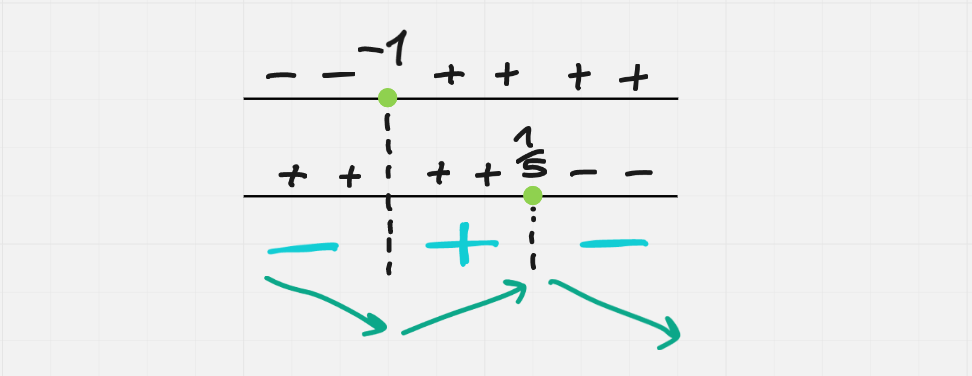
\includegraphics[width=\textwidth]{disequaz-giugno-2019.png}
	quindi $f'(x)\geq 0$ se e solo se $x\in [-1,0)\cup (0,\frac{1}{5}]$ (nota che zero è escluso perchè è punto di disconitinuità).
	\\In particolare, $x=-1$ è punto di minimo relativo, $x=\frac{1}{5}$ è punto di massimo relativo.

	\paragraph*{Grafico Qualitativo}
	Per tracciare il grafico, conosco i punti di discontinuità, i limiti e gli asintoti.
	\\Per comodità, trovo: $f(-1)=0$ e $f(\frac{1}{5})=-4$ e traccio il grafico:
	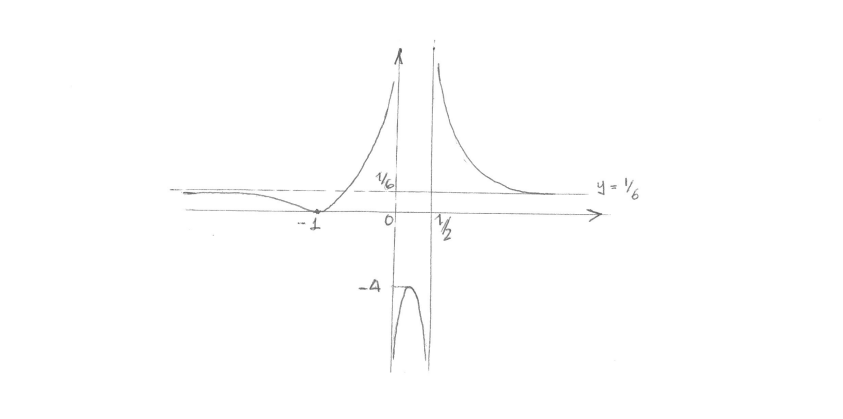
\includegraphics[width=\textwidth]{grafico-giugno-2019.png}
}
\domandaaperta{2}{
	Si enunci il teorema di esistenza del limite per successioni monotone.
	\\Data la successione:
	$$
	a_n = \ln(n+1)-\ln n = \ln(\frac{n+1}{n}) \text{ con } n\geq 1
	$$
	\textbf{i.} si verifichi, utilizzando la definizione, che è monotona (crescente o decrescente?);
	\\\textbf{ii.} si calcoli $\limite{n}{+\infty}(\ln(n+1)-\ln n)$
	\\\textbf{iii.} si calcoli la somma della serie $\serie{1}{+\infty}(\ln(n+1)-\ln n)$
}
\rispostaaperta{
	\paragraph*{Teorema di esistenza del limite:}
	Se una successione è monotona crescente allora il limite esiste e coincide con l'estremo superiore della successione.
	\\Se invece è monotona decrescente allora il limite esiste e coincide con l'estremo inferiore della successione.
	\paragraph*{i}
	Si vuole dimostrare che la successione sia monotona (crescente o decrescente).
	\\Notiamo che la successione si può semplificare in: $a_n=\ln(1+\frac{1}{n})$, il che ci rende le cose molto più facili:
	\\intuitivamente notiamo che $a_{n+1}<a_n$, quindi:
	$$a_{n+1} = \ln(1+\frac{1}{n+1}) < ln(1+\frac{1}{n}) = a_n$$
	e, siccome $\frac{1}{n+1}<\frac{1}{n}$ e la funzione logaritmo è crescente ($\ln(n)<\ln(n+1)$)
	ne consegue che la serie $\{a_n\}$ è \emph{Monotona Decrescente}.
	\paragraph*{ii}
	$limite{n}{+\infty} a_n = \ln(1+\frac{1}{n}) = \ln(1) = 0$.
	\\Volendo si può dire anche che per un $x\to0$ il logaritmo di $(1+x)$ è asintotico ad $x$, in questo caso quindi sarebbe asintotico a $\frac{1}{n}$, ovvero 0.

	\paragraph*{iii}
	La serie $a_n$ è a termini positivi e $\ln(n+1) - \ln(n) \sim \frac{1}{n}$ (vedi sopra), pertanto è divergente ($+\infty$)s.
}

\section{Giugno 2020}
\domanda{1}{La funzione $f:\R \to \R$ definita da $f(x)=\begin{cases}e^x & x>0 \\ x+2 & x\leq 0\end{cases}$ è}
\risposta{Suriettiva ma non Iniettiva}
\spiegazione{
	La funzione è \emph{suriettiva} perchè riempie tutto $\R$.
	Per controllarlo basta vedere i grafici dei due segmenti della funzione.
	\\Non è iniettiva invece perchè ci sono dei punti del codomino "raggiungibili" con due $x$ diverse.
	Per verificarlo basti vedere che nel grafico della funzione id due segmenti si accavallano su alcuni valori di $y$.
}

\domanda{2}{Siano $f(x) = e^{\sqrt{x}}$ e $g(x)= \ln(1+x)$. Allora $(g \circ f)$}
\risposta{è definita per ogni $x\geq 0$}
\spiegazione{$g\circ f = g(f(x)) = ln(1+e^{\sqrt{x}})$, quindi bisogna vedere dove è definita quella funzione.
\\Sappiamo che l'argomento di una radice va posto maggiore o uguale a zero, e quello di un logaritmo va posto maggiore di 0}

\domanda{3}{La somma della serie $\serie{1}{+\infty} e^{1-2n}$ vale}
\risposta{$\frac{e}{e^2-1}$}
\spiegazione{
La serie si può riscrivere come:
\\$\serie{1}{\infty} e^{1-2n} = e\sum (\frac{1}{e^2})^n$
\\Essendo una serie geometrica con argomento minore del modulo di 1, si può risolvere con la formula risolutiva.
Siccome però la serie parte da 1, bisogna togliere la somma con n=0 (moltiplicata per la costante $e$), quindi:
\\$= e \frac{1}{1-\frac{1}{e^2}} -e = \frac{e}{1-\frac{1}{e^2}}-e 
= \frac{e}{\frac{e^2-1}{e^2}}-e 
= e\frac{e^2}{e^2-1}-e = \frac{e^3}{e^2-1}-e = \frac{e^3-e^3+e}{e^2-1}
=\frac{e}{e^2-1}
$
\\nota che il $-e$ sarebbe $-e\cdot(q)0$
}
\domanda{4}{Sia $f:\R \to \R$ la funzione definita da $f(x) = \int_{1}^{x} t^2 e^{\sqrt[3]{t}} dt$. Allora:}
\risposta{$f$ è Crescente}
\irrisolta

\domanda{5}{$\limite{n}{+\infty} \frac{n^2 \ln^3 n - n^3 \ln^2 n +4 \arctan n}{n^3 \ln^2 n - n^2 \ln^5 n- e^{-n^2}}$ vale:}
\risposta{-1}
\spiegazione{$\frac{n^2 \ln^3 n - n^3 \ln^2 n +4 \arctan n}{n^3 \ln^2 n - n^2 \ln^5 n- e^{-n^2}} \sim \frac{-n^3 \ln^2 n}{n^3 \ln^2 n} = -1$}

\domanda{6}{Il massimo dell'insime $A = {\frac{2+(-1)^n}{2^n+(-1)^{n+1}}}$ è}
\risposta{1}
\spiegazione{per $n=2$ l'insieme vale 1, mentre per tutti gli altri valori di n è minore.}


\domanda{7}{sia $f(x) = \arctan(\sqrt{x})$. Allora $f'(1)=$}
\risposta{Nessuna delle precedenti ($\frac{1}{4}$)}
\spiegazione{Trovo la derivata della funzione:
	\\$f'(x) = \frac{1}{1+x} \cdot \frac{1}{2\sqrt{x}} = \frac{1}{2\sqrt{x}(1+x)}$. La derivata vale in $x=1$:
	$f'(1) = \frac{1}{4}$}

\domanda{8}{Sia $f$ definita e continua su [a,b]. Allora}
\risposta{Assume il valore $\frac{f(a)+f(b)}{2}$}
\spiegazione{Non ho trovato nessuna definizione che giustifichi questa cosa, ma da Telegram mi dicono:
	Se una funzione è continua in un intervallo ed ho $y_1 = f(a)$ e $y_2 = f(b)$ allora la funzione può assumere tutti i valori tra $y_1$ e $y_2$.
	$\frac{f(a)+f(b)}{2}$ se lo guardi nell'asse delle y è un valore compreso tra $f(a)$ e $f(b)$.
	\\Un'altra risposta corretta potrebbe essere: Assume tutti i valori tra $f(a)$ e $f(b)$.
}

\subsection{Domande Aperte}
\domandaaperta{1}{
	Si determinino $a$ e $b$ affinchè la funzione:
	\begin{equation*}
		f(x)= \begin{cases}
			a\frac{\ln(x-1)}{x-2} +bx & x>2\\
			2x^2-2x+1 &0 \leq x \leq 2\\
			a(x+1)+3\frac{e^{bx}-1}{x} & x<0
		\end{cases}
	\end{equation*}
	Sia continua in $\R$
}
\domandaaperta{2}{
Data la funzione $f(x) = xe^{x-x^2+4}$
}
\domandaaperta{a}{
Si calcolino $\limite{x}{-\infty}f(x)$ e $\limite{x}{+\infty} f(x)$
}
\rispostaaperta{
$\limite{x}{+\infty} f(x) = 0^+$, perchè $e^{x-x^2+4} \sim e^{-x^2}$, quindi $+\infty \cdot 0 = 0^+$.
$\limite{x}{-\infty} f(x) = 0^-$, perchè $e^{x-x^2+4} \sim e^{-x^2}$, quindi $-\infty \cdot 0 = 0^-$.
}
\domandaaperta{b}{
Si determini il più ampio intervallo del tipo ($-\infty,k)$ su cui $f$ è monotona e si specifichi se $f$ è crescente o decrescente
}
\rispostaaperta{Per controllare la monotonia, faccio la derivata di $f(x)$ e la pongo $\geq 0$:
\\$f'(x)= e^{x-x^2+4}+xe^{x-x^2+4}-2x^2e^{x-x^2+4} =e^{x-x^2+4}(1+x-2x^2)$.
\\$f'(x)\geq 0 \to [-\frac{1}{2},1]$
\\$f'(x)\leq 0 \to (-\infty,-\frac{1}{2}]\cup[1,+\infty)$, di conseguenza l'intervallo più alto in cui $f$ è monotona è:
$(-\infty,-\frac{1}{2}]$ in cui è decrescente.
}
\domandaaperta{c}{
	L'insieme immagine $Im(f)$ è:
}
\rispostaaperta{
	Per trovare l'insieme immagine della funzione si può guardare il grafico della funzione (che in questo caso sarebbe una menata) oppure procedere un po a ragionamento.
	\\Tramite lo studio della monotonia sappiamo che la funzione ha punto di minimo a $x=-\frac{1}{2}$ e di massimo a $x=1$.
	Sappiamo anche che a sinistra la funzione va ad "appoggiarsi" a $0^-$ e da destra si "appoggia" a $0^+$.
	\\Di conseguenza riusciamo a capire che l'immagine della funzione è $[f(-\frac{1}{2}), f(1)]$, quindi $[-\frac{1}{2}e^{\frac{13}{4}}, e^4]$ 
}
\domandaaperta{3}
{Data la funzione $f(x) = \ln(1+2x)-2\sin x-6x^3$}
\domandaaperta{a}{Il polinomio di McLaurin del terzo ordine per $f$ è:}
\rispostaaperta{Per calcolare il polinomio di McLaurin del terzo ordine devo trovare la derivata prima, seconda e terza di $f(x)$ e il loro valore in $x=0$:
$$f'(x)= \frac{2}{1+2x} - 2\cos x - 18x^2 \implies f'(0) = 0$$
$$f''(x)=-\frac{4}{(2x+1)^2} + 2\sin x - 36x \implies f''(0)=-4$$
$$f'''(x)=\frac{16}{(2x+1)^3}+2\cos x -36 \implies f'''(0)=-18$$
Uso la formula per calcolare il polinomio di McLaurin:
$$P= -2x^2 -3x^3$$
}
\domandaaperta{b}{$\int^{2}_{0} f(x) dx$ vale: }
\domandaaperta{4}{Data la successione $\{a(n)\}_{n\in\N}$, si enunci, con le debite ipotesi, il criterio del rapporto per successioni.
\\Utilizzando tale criterio, si calcoli:
$$\limite{n}{+\infty} \frac{(2n)!}{(n+4)!}$$
}

\section{Giugno 2021}
\domanda{O1}{Sia $f:\R \to \R$ definita da $f(x) = x^3 + 4x$. sull'intervallo $I = (-1,1)$ la funzione $f$ è:}
\spiegazione{Studiare CONCAVITA' e CONVESSITA'}
\irrisolta
\domanda{O2}{La somma della serie $\serie{0}{+\infty} (\frac{2}{3})^{2n}$ vale}
\risposta{$\frac{9}{5}$}
\spiegazione{La serie è simile a una geometrica, però c'è quel $2n$ da mandare via, quindi:
$$ (\frac{2}{3})^{2n}= [(\frac{2}{3})^{2}]^n = (\frac{4}{9})^{n}$$
Ora è una normale serie geometrica con argomento $< |1|$, che risolta con la formula $\sum (q)^n = \frac{1}{1-q}$ ci da $\frac{9}{5}$
}
\domanda{O3}{Siano $f(x) = \ln(x^2+1)-1$ e $g(x) = |x+1|$. Allora $(g \circ f)(x) = $}
\risposta{$ln(x^2 + 1)$}
\spiegazione{
	Sappiamo che $(g \circ f)(x) = g(f(x))$, quindi lo svoglimento è banale. Segnalo però che $|ln(x^2+1)| = ln(x^2+1)$, perchè il logaritmo ha dominio maggiore di 0, e in questo caso il suo argomento è sempre maggiore di 0, quindi le due funzioni si equivalgono.
}
\domanda{O4}{L'estremo superiore dell'insieme $A={\frac{1}{n+1} +2^{1-2n}, n= 1,2,...}$ è}
\risposta{1}

\domanda{O5}{La funzione $f:\R \to \R$ definita da $f(x) = \begin{cases} e^{-x} & x>0 \\ x^2-1 &x\leq 0 \end{cases}$ è}
\risposta{Nè suriettiva nè iniettiva}
\spiegazione{
	$e^{-x} = \frac{1}{e^x}$, che parte da vicino a uno e tende a 0.
	\\$x^2-1$ è invece una funzione che parte da -1 e va verso l'alto.
		\\Essendo la funzione definita in $\R$, ed essendo il minimo -1, la funzione non è suriettiva.
	Visto che la seconda parte da -1 e va verso l'alto, mentre la prima parte da 1 e va verso 0, si incrociano sicuramente, rendendo la funzione non iniettiva.
}
\domanda{O6}{L'integrale definito $\int_{0}^{2} \frac{x}{x^2+1} dx$ Vale:}
\risposta{$\frac{ln(5)}{2}$}
\spiegazione{Questa è una funzione razionale che può essere semplicemente trasformata in una del tipo $\frac{f'(x)}{f(x)}$ (che può essere risolta ed equivale a $\ln|f(x)|$) moltiplicando e dividendo per due, quindi:
	\\$\int  \frac{x}{x^2+1} = \frac{1}{2} \int \frac{2x}{x^2+1} = \frac{1}{2} \ln(x^2+1)$
		\\$[\frac{1}{2} \ln(x^2+1)]_{0}^{2} = \frac{ln(5)}{2}$
}

\domanda{O7}{$\limite{n}{+\infty}(\ln n - \sqrt{n}+3e^{-n} +\sin n^2)$ Vale:}
\risposta{$-\infty$}
\spiegazione{Bisogna trovare il limite più importante e in questo caso abbiamo:
\begin{itemize}
	\item $+\sin n^2$ che oscilla tra $0$ e $1$, quindi ignorabile
 \item $+3e^{-n}$ che è infinitesimo, quindi ignorabile
\end{itemize}
Ci restano solo  $\ln n - \sqrt{n}$, entrambi infiniti, ma contando che la radice è un infinito di ordine maggiore, vince lei e diventa $-\infty$
	}
\domanda{O8}{Siano $f,g : \R \to \R$ derivabili. se $f(2) = -2, f'(2)=4,g'(-2) = -4}$, allora $(g\circ f)'(2)$ Vale:

\subsection{Domande Aperte}

\domandaaperta{1}{Sia $\serie{1}{+\infty}(n^{\frac{1}{n}}-1)^n$}
\domandaaperta{a}{Per studiare la serie uso il criterio:}
\domandaaperta{b}{Applicando tale criterio ottengo il limite:}
\domandaaperta{c}{Qual'è il valore di tale limite? la serie converge o diverge?}

\domandaaperta{2}{Data la funzione $f(x) = x\sin x^2$}
\domandaaperta{a}{Si scrivano tutte le primitive}
\domandaaperta{b}{Si determini la primitiva $\phi$ tale che $\phi(\sqrt{3\pi/2}) = 0$}
\domandaaperta{c}{si calcoli $\int^{\sqrt{2\pi}}_{\sqrt{3\pi/2}}f(x)dx$}

\domandaaperta{3}{Devo ancora scriverla lol}

\chapter{Cheatsheet}
\section*{Serie}
\paragraph*{Serie Armonica Generalizzata}
\begin{equation*}
	\sum \frac{1}{n^\alpha} \begin{cases}
		\text{Diverge} & \alpha\leq 1\\
		\text{Converge} & \alpha> 1
	\end{cases}
\end{equation*}
\paragraph*{Serie Geometrica}
\begin{equation*}
	\serie{0}{+\infty} q^n \begin{cases}
		\text{Diverge} & q\geq 1\\
		\text{Converge} & -1<q<1 \\
		\text{Irregolare} & q\leq 1
	\end{cases}
\end{equation*}
\section*{Limiti}
\paragraph*{Ordine degli infiniti}
Nel calcolo dei limiti, quando bisogna trovare l'infinito di ordine maggiore:
$$ \log_ax\ll x^b\ll x^c\ll d^x\ll g^x\ll x^x $$
con $a>0 \wedge a\neq 1$, $0<b<c$, $1<d<g$
\nb{la radice è "più grande" del logaritmo}
\end{document}